\documentclass[letterpaper]{article}

\usepackage{hw}
\usepackage{bm}
\usepackage{amsmath}
\usepackage{graphicx}
\usepackage[colorlinks=false,urlcolor=blue]{hyperref}
\usepackage{multicol}
\usepackage{paralist}
\usepackage{todonotes}
\usepackage{booktabs}
\usepackage{enumitem}
\usepackage{cleveref}
\usepackage{pdfpages}
\usepackage{fancyhdr}
\usepackage{fancyvrb}
\usepackage{tikz}
\usetikzlibrary{arrows}
\usepackage{graphicx}
\usepackage{listings}
\usepackage{color}
\usepackage{subfig}

\usepackage{amssymb}
\usepackage{amsmath}
\usepackage{tikz}
\usetikzlibrary{matrix,calc}

\newenvironment{smallarray}[1]
  {\gdef\MatName{#1}\begin{tikzpicture}
    \matrix[
    matrix of math nodes,
    row sep=-\pgflinewidth,
    column sep=-\pgflinewidth,
    nodes={inner sep=1pt,rectangle,text width=2mm,align=center},
    text depth=0mm,
    text height=2mm,
    nodes in empty cells
    ]  (#1)}
  {\end{tikzpicture}}
\def\MyZ(#1,#2){%
  \draw ([xshift=-3.6pt,yshift=3.6pt] $ (\MatName-#1-#2)!0.5!(\MatName-\the\numexpr#1+1\relax-\the\numexpr#2+1\relax) $ ) rectangle ([xshift=3.6pt,yshift=-3.6pt] $ (\MatName-#1-#2)!0.5!(\MatName-\the\numexpr#1+1\relax-\the\numexpr#2+1\relax) $ );
}

\DeclareCaptionType{copyrightbox}
\captionsetup{font=small}
\captionsetup{labelfont=bf}
\captionsetup[subfloat]{font=scriptsize}
\captionsetup[subfloat]{farskip=5pt}
\captionsetup[subfloat]{captionskip=1pt}
\captionsetup[table]{belowskip=0pt}

\crefname{listing}{Program-code}{Program-codes}  
\Crefname{listing}{Program-code}{Program-codes}

%\DeclareMathOperator*{\argmin}{arg\,min}
%\DeclareMathOperator*{\argmax}{arg\,max}

\lstdefinestyle{customc}{
  belowcaptionskip=1\baselineskip,
  breaklines=true,
  xleftmargin=\parindent,
  language=C,
  showstringspaces=false,
  basicstyle=\footnotesize\ttfamily,
  keywordstyle=\bfseries\color{green!40!black},
  commentstyle=\itshape\color{purple!40!black},
  identifierstyle=\color{blue},
  stringstyle=\color{orange},
}

\lstdefinestyle{customasm}{
  belowcaptionskip=1\baselineskip,
  frame=L,
  xleftmargin=\parindent,
  language=[x86masm]Assembler,
  basicstyle=\footnotesize\ttfamily,
  commentstyle=\itshape\color{purple!40!black},
}

\lstset{escapechar=@,style=customc}

\newcommand{\email}[1]{\href{mailto:#1@cs.cmu.edu}{#1}}

\begin{document}
\title{Optimizing Matrix Operations Using Novel DRAM
  Access Primitives}
 \author{}
\date{}
\maketitle
\begin{center}
  \textsc{\large CMU 15-745: Optimizing Compilers (Spring 2015)} \\
  \vspace{1em}
  \textsc{\large Final Report} \\
  \vspace{1em}
  \centerline{\large{Joy Arulraj (\email{jarulraj}), Anuj Kalia
    (\email{akalia})}, Jun Woo Park (\email{junwoop}) }
  \vspace{1em}
\end{center}

\section{Abstract}

Traditionally, when an application requests a set of different rows
residing on the same memory bank, the memory access latency is
increased due to DRAM row-buffer conflicts.
These row-buffer conflicts can be reduced by interleaving
consecutively addressed data locations across memory banks, so that
the requests are spread across different banks.
Software systems, therefore, strive hard to lay out their data structures
to generate access patterns that can be served efficiently by
the DRAM chips.
For instance, DBMSs targeting analytical workloads use a columnar data
layout so that values in the same tabular column are stored in
consecutively addressed data locations~\cite{col1}.

The design complexity of software systems can be significantly
reduced in future DRAM chips using novel access primitives that can
support both row and columnar access patterns efficiently.
This is feasible by appropriately laying out the data and transforming
the DRAM access methods.
In this project, we focussed on automatically
transforming the software access patterns to leverage these
DRAM access primitives during compilation time.
We developed a DRAM access cost model to select the appropriate DRAM
access primitive for different patterns. We then
analyze the software access patterns in our compiler pass and then
transform the code to make use of these access primitives.
Our evaluation of the performance impact of these transformations in
a matrix library showed that TODO.

\section{Introduction}

DRAM access patterns significantly impact the performance of memory-bound
applications. The delay incurred while handling a cache miss is not
constant as the access latencies within DRAM are not uniform~\cite{dram1}.
DRAM is organized as a set of banks, each of which is made up of multiple
chips. Consecutive memory addresses are interleaved evenly across the
DRAM banks. Each bank has a row-buffer that is used to speed up DRAM
accesses. When the application requests for a page in a bank, the page
is first fetched into the bank's row buffer. Then, it is sent to the
the application. If the application happens to request for a page that
is already present in the row buffer, it is termed as a \textit{row-buffer
hit}. This results in the minimal DRAM access latency i.e. one memory
cycle.
However, if the page is not present in the row buffer, then the appropriate row
in the DRAM bank needs to be activated before the requested page can be loaded into
the row buffer and returned to the application. This event is referred to as a
\textit{row buffer miss}.

Programmers strive hard to lay out their application data structures
to generate access patterns that can be served efficiently by the DRAM chips.
For instance, DBMSs targeting analytical workloads use a \textit{pure-columnar}
data layout so that values present in the same tabular column are stored
in consecutively addressed data locations~\cite{col1,raman13,ailamaki02}. This
helps spread the DRAM accesses to multiple DRAM banks that can serve the requests in
parallel. Thus, the application can better utilize the available DRAM
bandwidth.

To give a concrete example, we compare the average time taken to compute the
sum of a row and sum of a column in a matrix laid out in row-major order.
The results are shown in ~\cref{fig:perf}.
We observe that summing a row in this case is 2--4$\times$ faster than the
columnar sum operation.

\begin{figure*}[ht]
	\centering
	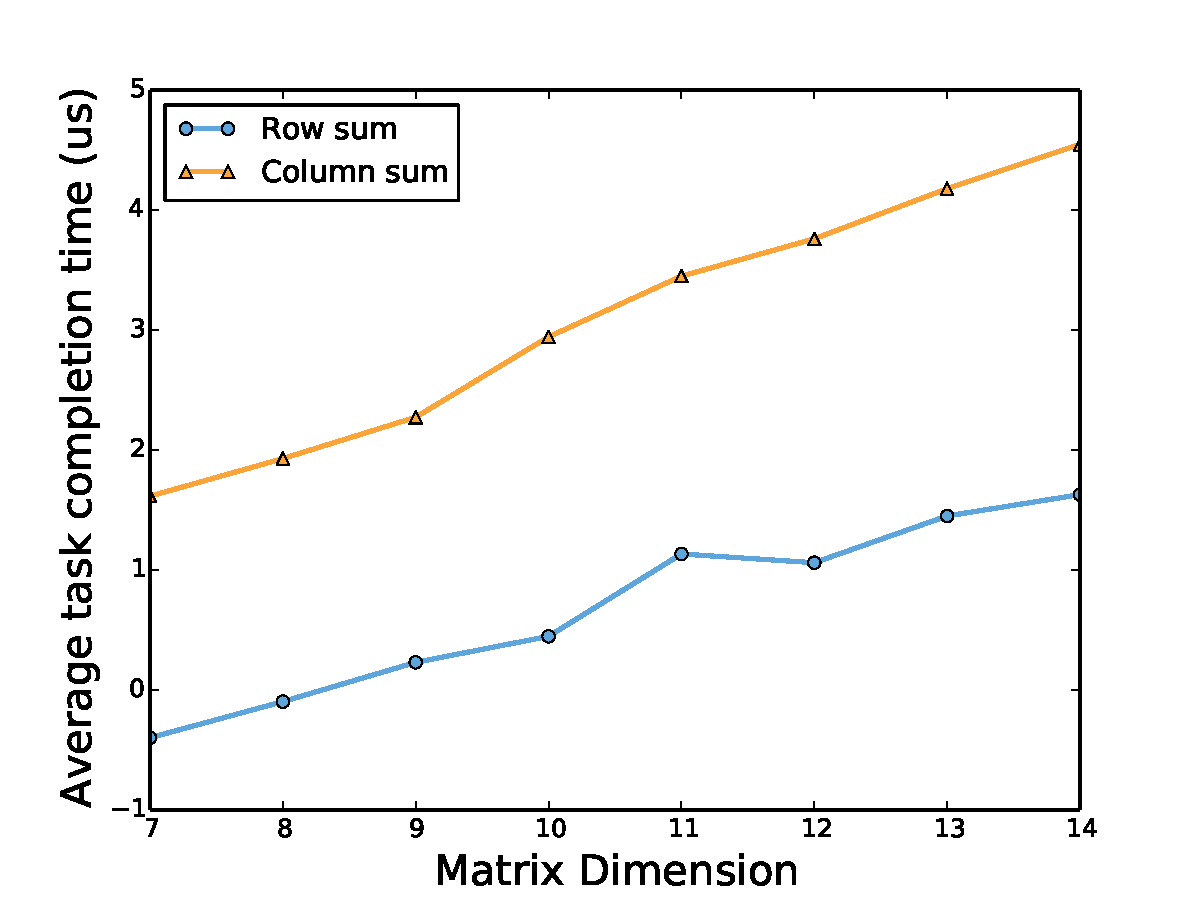
\includegraphics[scale=0.35]{images/rowmajor}
	\caption{Performance comparison of row and column oriented access patterns.
	The dimension attribute along the x-axis refers to the $\log_2$ of
	the length of the two-dimensional square matrix. }
	\label{fig:perf}
\end{figure*}

\subsection{The Problem}

In this work, we focus on applications that have complex workloads with
mixed DRAM access patterns. For instance, in a hybrid transaction and
analytical processing (HTAP) workload~\cite{grund10}, the DBMS needs to
access both the tuples and columns of a table efficiently. Irrespective of
whether the DBMS uses a pure-row or pure-columnar layout, one of the two
access patterns has to suffer from poor DRAM performance. For instance, assume
that the DBMS uses a pure-row layout and that the size of each tuple is one
cacheline (64 bytes).
When serving an analytical query that needs to sum up the values in a
particular column, we need to access only that part of the tuple
in all the tuples in the table.
This means that we would like to access only part of a cacheline.
This is however not feasible in current hardware, as the data is laid
out in tuple-major order.

In future hardware systems, we anticipate that we will have new DRAM access
primitives that allow us to access parts of a cacheline and not just
entire cachelines.
These primitives will allow the application to read a cacheline
composed of data stored in different DRAM rows by specifying
an DRAM \textit{access pattern}. This is illustrated in ~\cref{fig:primitives}.
Consider a 4$\times$4 toy matrix. In the default row-major layout,
fetching the first column will require four DRAM read operations as
they will be serialized at the same bank. If we \textit{shuffle}
the tile to DRAM row mapping as shown below, we observe that we can
access both the first row (cacheline 1) and first column (denoted by, say,
cacheline 1.2) using a single DRAM read operation.
This effectively allows us to retrieve the required data (for instance, a column
in a matrix) in fewer DRAM operations compared to existing DRAM access primitives.
Therefore, we can achieve (1) lower DRAM latency, (2) more efficient DRAM
bandwidth utilization, and (3) lower energy consumption.

\begin{figure*}[ht]
	\centering
	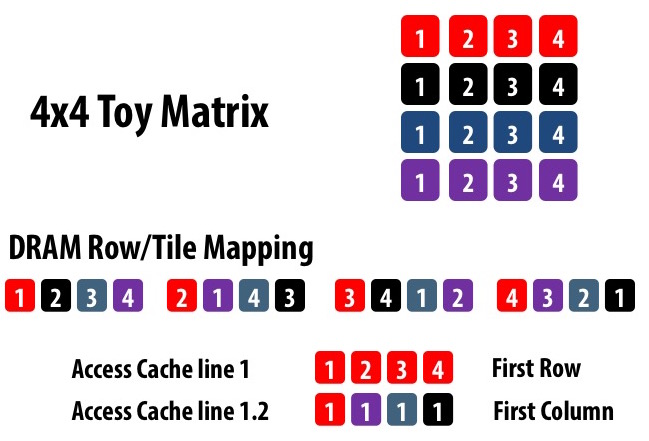
\includegraphics[width=0.8\textwidth]{images/primitives}
	\caption{Novel DRAM access primitives that allow the application to read
	both a column or a row in a small matrix in a single DRAM read operation.}
	\label{fig:primitives}
\end{figure*}


The problem we address in this work involves designing a compiler pass that
allows us to \textit{automatically} identify the application's access
patterns and transforms the program to make use of these novel DRAM access
primitives.
This reduces the burden on the programmer and thereby simplifies the adoption
of these DRAM access primitives.

\subsection{Our Approach}

At a high level, we decouple the problem into two subproblems:

\begin{itemize}
  \item {We need to figure out the different application access patterns}
  \item {We then need to map the application access patterns to make use of
  underlying DRAM access primitives.}
\end{itemize}

We have implemented an LLVM pass that analyses data structure access patterns
and uses a DRAM access cost model to map the access pattern to an optimal DRAM
access primitive.
Our pass can successfully handle arbitrary data structure access patterns
over multi-dimensional arrays of primitive data types as well as structures.

\subsection{Related Work}

We have gone through several traditional papers on DRAM access
primitives and data locality~\cite{dram1,dram2,dram3}.
As the DRAM primitives we are targeting in this work are not currently
available, we could not find more relevant literature.
However, there has been a lot of prior work on handling hybrid application
patterns with existing hardware constraints, particularly in the
area of database systems.
Copeland et. al.~\cite{Copeland85} presented the advantages of a storage model
based on decomposition over conventional row-oriented storage models.
More recently, HYRISE~\cite{grund10} and MonetDB/X100~\cite{monetdb} systems 
have been designed to handle hybrid and analytical query workloads respectively
on existing memory subsystems.
In particular, the X100 engine~\cite{Zukowski05} introduced in-cache vectorized 
processing to balance between the column-at-a-time execution in MonetDB and the
traditional tuple-at-a-time Volcano pipelining model.

\subsection{Contributions}

We make the following contributions in this project:

\begin{itemize}
  \item {We implemented an LLVM pass that determines the different data
  structure access patterns by an application.}
  \item {We developed a basic DRAM access cost model that allows the compiler to
  map the application access pattern to the most optimal DRAM access pattern.}
  \item {We illustrate the performance benefits of these novel DRAM access primitive
  through a quantitative evaluation on different workloads in a custom matrix
  library.}
\end{itemize}

\section{Matrix Access Pattern Analysis}

The goal of this analysis is to identify the different application access
patterns and then map then onto an efficient DRAM access primitive to improve
cache and memory subsystem performance. In this section, we will first present
the compiler pass and then describe the DRAM access cost model that we leverage
in our mapping function.

\subsection{LLVM Pass}

We define an application's data structure access pattern in terms of two 
parameters : (1) \textit{stride}, and (2) \textit{offset}. 
For instance, consider an array of structures, each of which contains two
integer fields. 
Then, if the application accesses the second field in all the structures 
in the array in a loop, we denote that access pattern as $\{4,+,8\}$. 
Here, the first member is the offset and the second element is the stride.

We implemented a compiler pass that analyses our matrix library automatically
to determine the stride and offset of the application's access patterns.
We assume that the programmer annotates the data structures that should
be analysed using LLVM annotations.
In theory, we can apply our analysis on all loads and stores in the program.
However, we wanted to restrict our analysis to important data structures
as that approach is more practical.
Further, we also focus only on memory accesses within \textit{loops} in the 
application. This is because we believe that optimizing these memory accesses
with the novel DRAM access primitives will be sufficient to realize
significant application speedups.

This compiler pass consists of three stages :
\begin{itemize}
  \item{We first parse the programmer annotations to determine the critical data
  structures.}
  \item{Then, for each loop in the program, we analyze the loads and
  stores associated with these data structures to determine the access pattern.}
  \item{Finally, we use the cost model to map the access pattern to the
  relevant DRAM access primitive.}
\end{itemize}

We implemented the first stage using LLVM's support for data member annotations.
Then, we leveraged the scalar evolution (SCEV) analysis~\cite{llvm15} functions
in the second stage of the compiler pass.
These functions support the analysis of scalar expressions within loops and
help recognize general induction variables.
Given a program \textit{scope} and a register, we can use these functions to
obtain an expression that represents the register's evolution inside the scope.
We applied these functions to the load and store addresses of the annotated 
data structure within the scope of the innermost loop. We then parsed the
recursive expression and delinearized it to obtain the stride and offset
with which the application accesses the critical data structures in the loop.

The output of the compiler pass on a sample program is shown below :

\begin{lstlisting}[caption={Sample Input Program},label={lst:input}]

------------------------------------------------------------
INPUT PROGRAM
------------------------------------------------------------

void foo(long n, long m)  {
  __attribute__((annotate(``this is important''))) int A[n][m];
  
  struct key{
    char a;
    char b;
    char c;
  };
  __attribute__((annotate(``critical''))) struct key keys[100];

  char x;
  for (long i = 0; i < n; i++) {
    for (long j = 0; j < m; j++){
      A[i][j] = 0;
      A[j][i] = 0;
      x = keys[i].a;
      keys[i].b = x;
    }
  }
}
\end{lstlisting}

\begin{lstlisting}[caption={Analysis Output},label={lst:output}]

------------------------------------------------------------
ANALYSIS OUTPUT :
------------------------------------------------------------


Analysing function :: foo:

------------------------------
Annotations found :
------------------------------

tests/a.c:i32 5           
%vla = alloca i32, i32 %1, align 4    
this is important

tests/a.c:i32 13          
%keys = alloca [100 x %struct.key], align 1   
critical

------------------------------
Loads/Stores :
------------------------------

------------------------------
Instruction:   store i32 0, i32* %arrayidx6, align 4
------------------------------

Access Pattern :
{{0,+,(4 * %m)}<%for.cond>,+,4}<nw><%for.cond3>

Delinearized Access Pattern :
[{0,+,1}<nuw><nsw><%for.cond>][{0,+,1}<nuw><nsw><%for.cond3>]

------------------------------
Instruction:   store i32 0, i32* %arrayidx8, align 4
------------------------------

Access Pattern :
{{0,+,4}<nuw><nsw><%for.cond>,+,(4 * %m)}<%for.cond3>

Delinearized Access Pattern :
[{0,+,1}<nuw><nsw><%for.cond3>][{0,+,1}<nuw><nsw><%for.cond>]

------------------------------
Instruction:   %4 = load i8* %a, align 1
------------------------------

Access Pattern :
{0,+,3}<nuw><nsw><%for.cond>

------------------------------
Instruction:   store i8 %4, i8* %b, align 1
------------------------------

Access Pattern :
{1,+,3}<nw><%for.cond>

\end{lstlisting}

In the listing above, we observe that our pass can handle multi-dimensional
arrays of both primitive and aggregate data types. It can clearly distinguish
the row-oriented and colum-oriented access patterns \texttt{A[i][j]} and 
\texttt{A[j][i]}. In the former case, the access pattern is of the form :\\
  
\texttt{\{\{0,+,(4 * \%m)\}<\%for.cond>,+,4\}<nw><\%for.cond3>},\\

i.e. the accesses are row-oriented. In the latter case, the stride is larger and
the accesses are column-oriented. This is even more evident from the delinearized access
patterns, wherein the order of the for-loop conditions are inverted in the
two cases.

Similary, in the case of the array of structures, the offset of the first
and second character fields within the structure are distinguished. This is
evident in the \texttt{\{0,+,3\}<nuw><nsw><\%for.cond>} and
\texttt{\{1,+,3\}<nw><\%for.cond>} access patterns. 
We have successfully tested our compiler pass on more complex access patterns. 
Overall, we can effectively analyze the loads and stores associated with the
critical data structures using the pass.

\subsection{DRAM Access Cost Model}

\begin{figure*}[ht!]
	\centering
	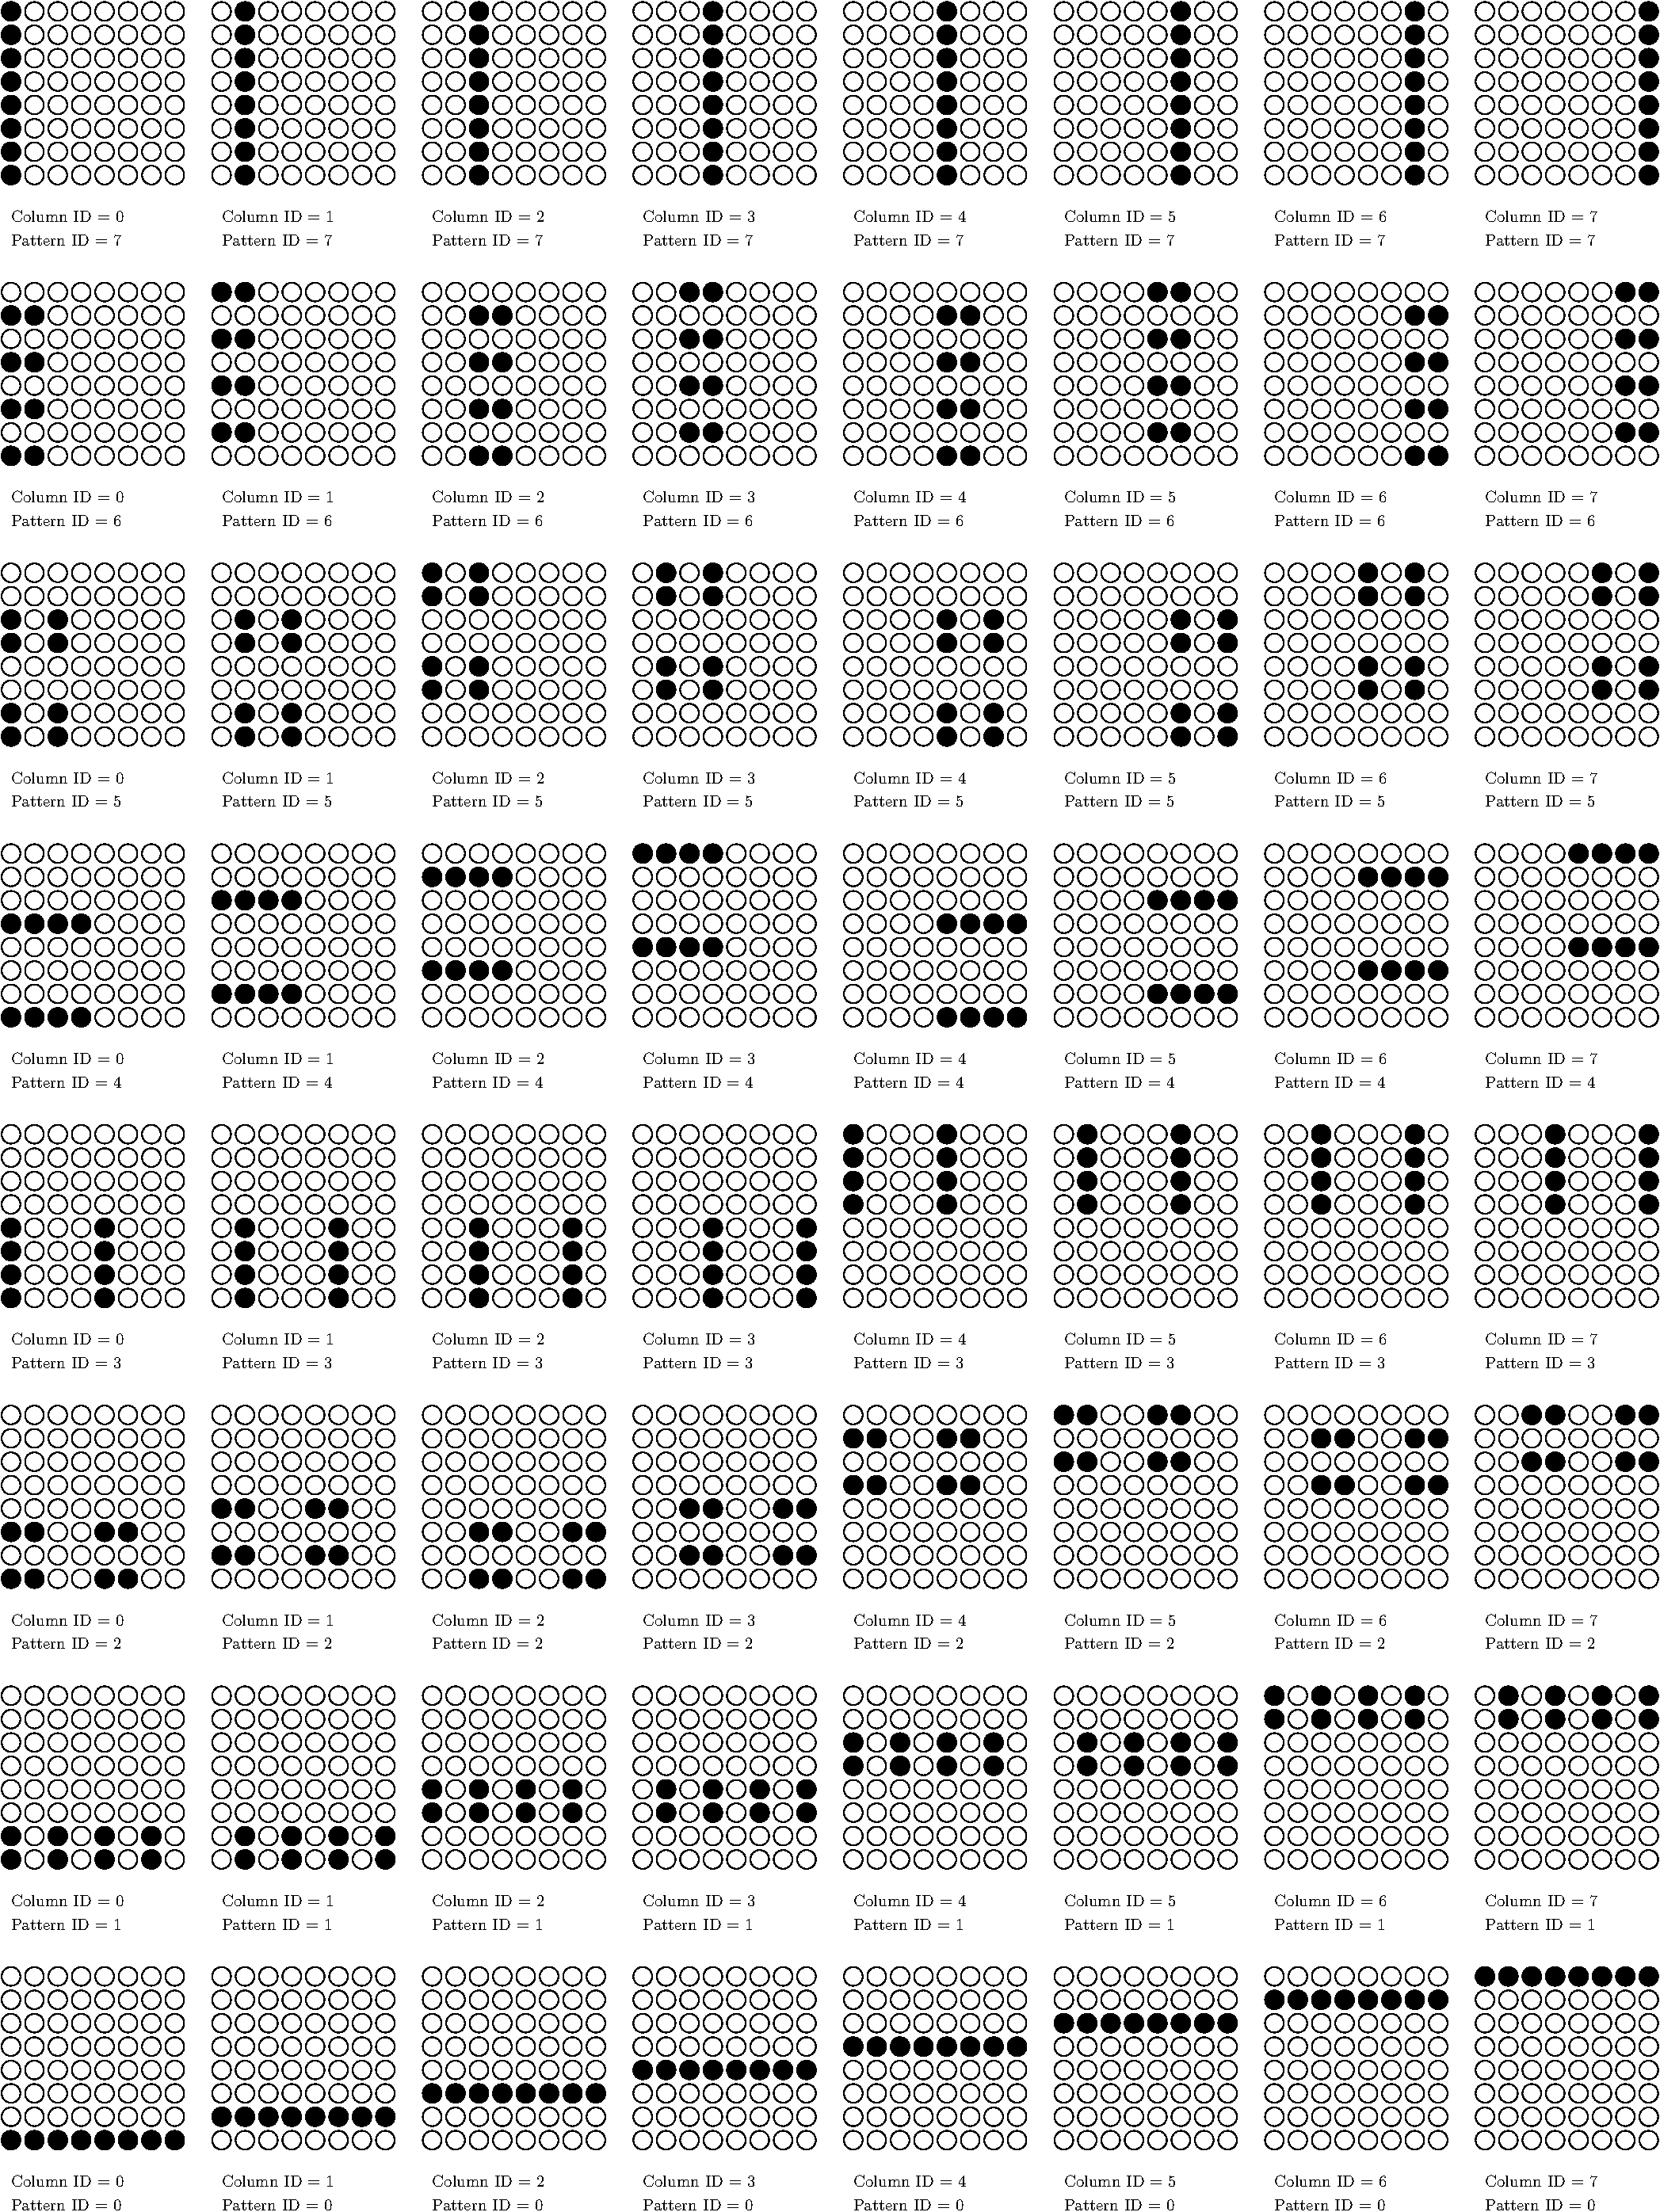
\includegraphics[width=0.9\textwidth]{images/pattern}
	\caption{List of possible patterns for a 8$\times$8 matrix with a given
	shuffling function. The column id refers to the cacheline being accessed. 
	The elements of the cacheline that are highlighted are returned to the
	application.}
	\label{fig:pattern}
\end{figure*}

We now describe the cost model we developed to help us map the
application's access patterns to the relevant DRAM access primitive.
To begin with, consider the list of possible patterns for 8$\times$8 
toy matrix with a given shuffling function shown in~\cref{fig:pattern}. 
We observe that there are $64$ total DRAM access patterns. 
In each case, the \textit{column id} refers to the cacheline being accessed,
while the \textit{pattern id} is the auxiliary information that we can 
supply using the novel DRAM access primitives.

The elements of the cacheline that are highlighted will be returned to the 
application that is requesting the desired cacheline and pattern id.
We note that using this tile to DRAM row mapping, we can access both
the first row and first column in the matrix in a single DRAM read operation.

\subsubsection{Simple Mapping Function}

Based on this observation, we started with a simple mapping function.
In the delinearized access pattern, if the innermost loop is the outer 
condition, then clearly it is column-oriented and will benefit from 
pattern id $7$. On the other hand, if the innermost loop is the inner
condition of the delinearized access pattern, then it will benefit
from pattern id $0$, the default pattern in current hardware systems.

Although this works well for relatively complex workloads comprising
of both row-oriented and column-oriented accesses to different 
data structures, this does not generalize to more complicated access
patterns. We therefore refined the cost model to take into account
other access patterns ranging from $1$ through $6$.

\subsubsection{Basic Cost Model}

In this model, for a given data structure, we first analyse all the cell
elements accessed by the set of all patterns in the loop. This is done
using the analysis described in previous subsection. We then compute
the difference between that tile and each of the available access patterns.
For instance, say the hybrid access pattern for the data structure looks
like this :

\begin{figure*}[ht!]
	\centering
	\begin{smallarray}{mat2}
	{
	\bullet & \bullet & \bullet & \bullet & \bullet & \bullet & \bullet & \bullet \\
	\bullet & \circ & \circ & \circ & \circ & \circ & \circ & \circ \\
	\bullet & \circ & \circ & \circ & \circ & \circ & \circ & \circ \\
	\bullet & \circ & \circ & \circ & \circ & \circ & \circ & \circ \\
	\bullet & \circ & \circ & \circ & \circ & \circ & \circ & \circ \\
	\bullet & \circ & \circ & \circ & \circ & \circ & \circ & \circ \\
	\bullet & \circ & \circ & \circ & \circ & \circ & \circ & \circ \\
	\bullet & \circ & \circ & \circ & \circ & \circ & \circ & \circ \\
	\bullet & \circ & \circ & \circ & \circ & \circ & \circ & \circ \\
	};
	\end{smallarray}
	\caption{Sample hybrid application access pattern.}
	\label{fig:hybrid}
\end{figure*}

The difference between the hybrid access pattern and pattern id 0, column id 0
is 6. Similarly, the difference between the hybrid access pattern and pattern id
7, column id 0 is also 6. Either of these DRAM access primitives will be
a good fit for the hybrid access pattern. In general, for two tiles
$\mathcal{T}_{a}$ and $\mathcal{T}_{b}$, each of dimensions $n$ $\times$ $m$, is 
given by :

$$\text{Basic Cost}(\mathcal{T}_{a}, \mathcal{T}_{b}) = \sum_{i=1}^{n}
\sum_{j=1}^{m} | \mathcal{T}_{a}[i][j] - \mathcal{T}_{b}[i][j] |$$

The lower the cost, the better the fit between the access primitive and the
hybrid access pattern. Although, this simple cost model  can handle more
complicated access patterns, including those resembling DRAM access patterns
$1$ through $6$, we realized that the model needs to be refined to consider
cacheline data alignment.

\subsubsection{Data Alignment Based Cost Model}

The key observation is that when the first cell in a given DRAM row is fetched,
the remaining cells in that row are also fetched into the row buffer.
Therefore, not all cells in the tile are equally important.
We can refine the cost model to handle data alignment in this manner.

For the tiles $\mathcal{T}_{a}$ and $\mathcal{T}_{b}$, each of dimensions $n$
$\times$ $m$, we first construct corresponding binary vectors $\mathcal{V}_{a}$
and $\mathcal{V}_{b}$, each of length $n$. For each row in the two tiles, 
if the sum of the elements in the row is non-zero, then the corresponding vector
element is set to one, i.e.

\[
\mathcal{V}_{a}[i] =
\begin{cases}
1 , & \text{if } \sum_{j=1}^{n} \mathcal{T}_{a}[i][j] > 0 \\
0 , & \text{otherwise} 
\end{cases}
\]

Now, we can define the cost as :

$$\text{Data Alignment Cost}(\mathcal{T}_{a}, \mathcal{T}_{b}) = \sum_{i=1}^{n} 
| \mathcal{V}_{a}[i][j] - \mathcal{V}_{b}[i][j] |$$

This refined model works well for cacheline alignment. However, we will need to
resolve ties between access primitives that have the same data aligment cost but
may not be equally good fits for the hybrid access pattern.
We therefore take both the basic cost and data alignment cost into consideration
to figure out the ideal access primitive for a given hybrid access pattern.
This is defined as :

\begin{align*}
\text{Weighted DRAM Access Cost}(\mathcal{T}_{a}, \mathcal{T}_{b}) 
&= \alpha \times \text{Data Alignment Cost}(\mathcal{T}_{a}, \mathcal{T}_{b})
+ \\
& (1-\alpha) \times \text{Basic Cost}(\mathcal{T}_{a}, \mathcal{T}_{b})
\end{align*}

Now, we can use the weighted DRAM access cost model to find the optimal DRAM
access primitive for a given hybrid application access pattern. Thus, to summarize,
we first analyze the loads and stores associated with the critical data
structures to determine the application's access patterns and then use the
cost model to map that access pattern to make use of the relevant DRAM access
primitive.

\section{Experimental Setup}

\textbf{Compiler Pass:} We implemented our compiler pass in the LLVM
3.5 framework. The pass analyses the application's data structure access
patterns with the help of scalar evolution-related (SCEV)
functions~\cite{llvm15}. 
We then use the cost model to find the optimal DRAM access primitive 
among the ones shown in~\cref{fig:pattern} for the given hybrid data access
pattern.

\textbf{Gem5:} Gem5 simulator is a configurable simulation framework that can
be used to emulate the novel DRAM access primitives. We used a modified version
of Gem5, that takes in \textit{pattern id} in the unused address bits from the
prefetch instruction to emulate the access pattern. The access function is 
shown below for clarity :

\begin{lstlisting}[caption={Gem5 DRAM Access Primitive
Simulation}]

#define PATTERN_ROW 0
#define PATTERN_COL 7

static __attribute__((aligned(512))) long table[];

// ACCESS PRIMITIVES
static long gather(long *table, int index, int pattern) {
    char *p = (char*)&table[index] + pattern;
    long result;
    // PREFETCH INSTRUCTION
    asm("prefetch %1\n" : "=a"(result) : "m"(*p) : );
    return result;
}

int main() {

	// ROW-ORIENTED ACCESS
	for (int i = 0; i < 16; i++) {
		printf("table[%2d] by tuple: %016lx\n", i, gather(table, i, PATTERN_ROW));
	}

	// COLUMN-ORIENTED ACCESS
	for (int i = 0; i < 16; i++) {
		printf("table[%2d] by field: %016lx\n", i, gather(table, i, PATTERN_COL));
	}

}
\end{lstlisting}
 
The changes in Gem5 are being made in tandem with this work. Due to functional
limitations of the current prototype, we were not able to obtain the statistics 
required for evaluating our benchmarks. 
We therefore decided to estimate the performance benefits directly on real
hardware using a matrix library that emulates different DRAM access primitives.
The specifications of the system that we used in our evaluation is shown
in~\cref{tab:spec}.

\begin{table}
    \centering
    \begin{tabular}{l|l}
    \textbf{CPU} & Intel Xeon CPU E5-2420 v2 $@$ 2.20GHz\\
    \textbf{Number of CPUs} & 12 \\
    \textbf{Threads per core} & 2 \\
    \textbf{L1d cache} & 32 KB \\
	\textbf{L1i cache} & 32 KB \\
	\textbf{L2 cache} & 256 KB \\
	\textbf{L3 cache} & 15 MB \\
  	\end{tabular}
    \caption{
        \textbf{System Specification} -- The hardware specification of the
        system used for evaluation }
    \label{tab:spec}
\end{table}

\section{Experimental Evaluation}

We evaluate potential performance impact of the novel DRAM access primitives by
comparing the time taken to complete the \textit{same task} using different
\textit{DRAM patterns ids} in our custom matrix library. 
The task involves performing a long series of reads and writes in a large array
at the tile-level granularity. We have a knob that allows us to adjust the
read-write ratio.
We then compare the performance obtained using different access patterns 
in the system after normalizing them with respect to the default pattern id $0$.

A high-level overview of the benchmark looks like this :

\begin{lstlisting}[caption={Benchmark}]

void Test(void * matrix, int pattern_id, int rd_wr_ratio, int scale) {
    StartTimer();
    
    for(k = 0 ; k < repeat; k++) {
        AccessMatrix(mat, pattern_id, rd_wr_ratio, scale);
    }

    StopTimer();
}

\end{lstlisting}

We vary the following parameters in our experiments :

\begin{itemize}
  \item \textbf{Pattern Id:} We implemented all the 8 access patterns depicted
  in~\cref{fig:pattern}.
  \item \textbf{Workload:} We consider four workloads (Read only, Read heavy,
Balanced, and Write Heavy) with the corresponding read-write ratio being 0,
0.25, 0.5, and 0.75 respectively. The \textit{AccessMatrix} function reads and writes
cells in different tiles of the matrix using the given pattern id based on the
read-write ratio in the generated workload.
  \item \textbf{Tile size:} This is the dimension of the square pattern matrix. 
  We considered the following values - 64, 128, 256, and 512.
\end{itemize}

We summarize our results in~\cref{fig:evaluation}, wherein we report the
normalized runtime with respect to the baseline row-major pattern \textit{P 0}.
Among all DRAM access primitives, we expected that the columnar access pattern
\textit{P 7} would perform the worst for our task, as we designed the task to
be ideally suited for the baseline DRAM access primitive.

\begin{figure*}[ht!]
    \centering
    \subfloat[64$\times$64 tile]{
	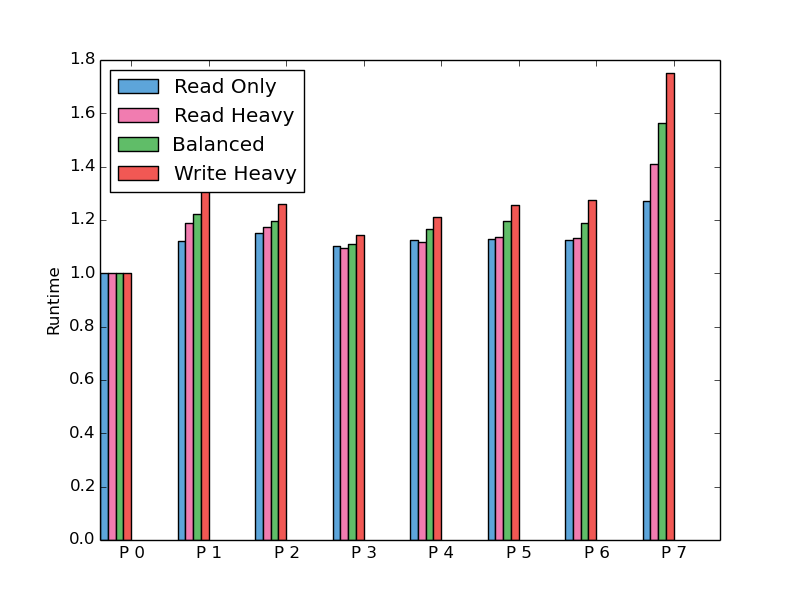
\includegraphics[width=0.5\textwidth]{images/64_runtime}
    }
    \subfloat[128$\times$128 tiles]{
	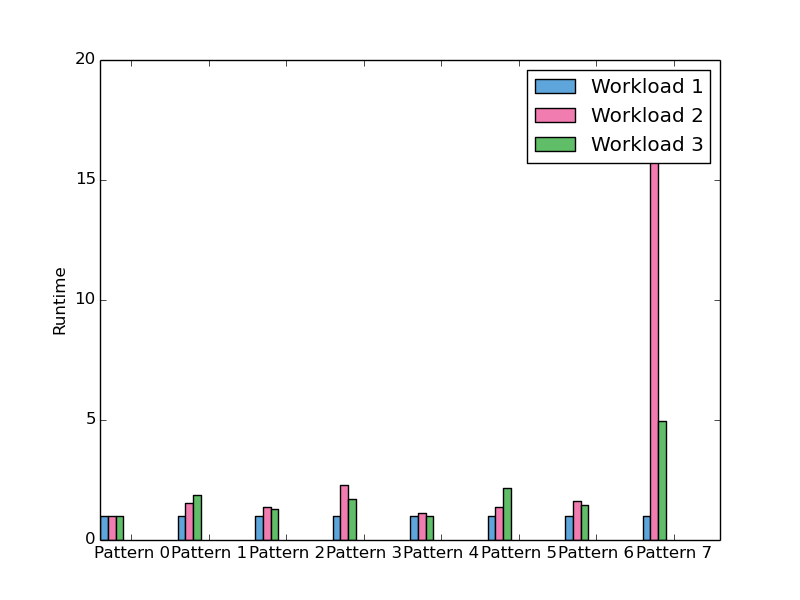
\includegraphics[width=0.5\textwidth]{images/128_runtime}
    }\\
    \subfloat[256$\times$256 tile]{
	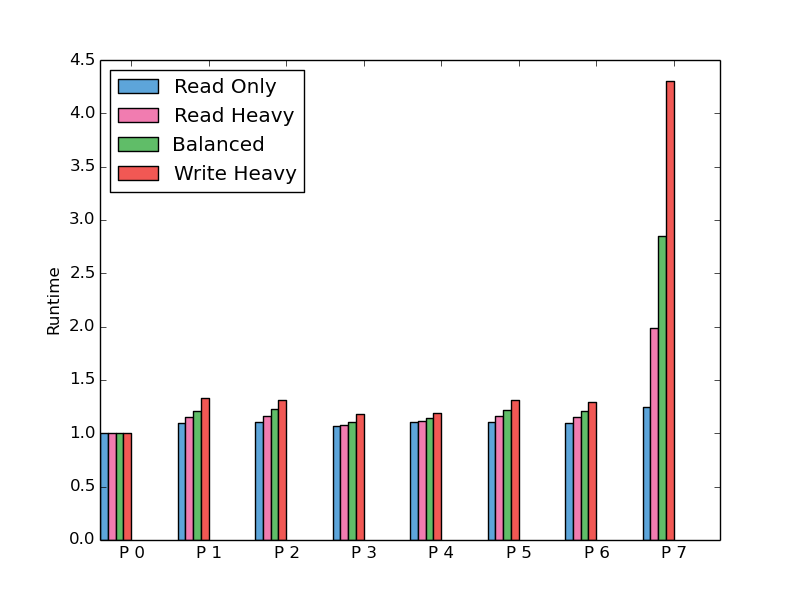
\includegraphics[width=0.5\textwidth]{images/256_runtime}
    }
    \subfloat[512$\times$512 tiles]{
	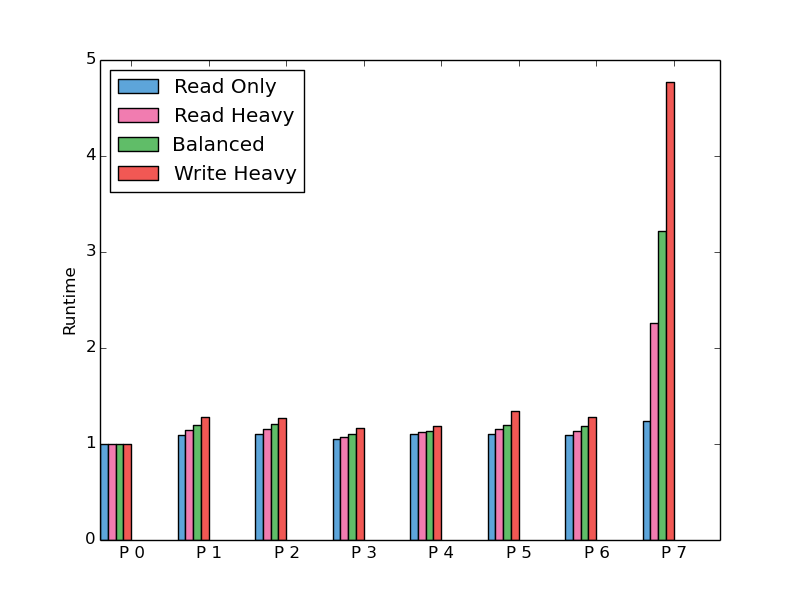
\includegraphics[width=0.5\textwidth]{images/512_runtime}
    }
    \caption{\textbf{Performance impact of DRAM access primitives} -- Evaluation
    of the normalized runtime incurred while running the same task using
    different DRAM access primitives. We consider four tasks (Read only, Read heavy,
    Balanced, and Write Heavy) and four tile dimensions.}

    \label{fig:evaluation}
\end{figure*}

The main takeaway was that the choice of DRAM access pattern has a strong
performance impact on the workload. In general, we observed that the other
DRAM access primitives performed worser than the baseline access pattern
on the task, to different extents.
This is in line with our expectation, as the task and the current memory
architecture is optimized for the default row-major DRAM access pattern.
We observed that the other access patterns incur significantly higher L1
data cache misses and this increases the normalized runtime of the workload.

Furthermore, we note that the performance degradation is more
pronounced in case of the write-intensive workloads (Balanced and Write-Heavy).
We attribute this to the fact that write operations will need to 
fetch the data and also write back the modifed contents back to memory,
unlike the read operations. This increases the number of row-buffer
conflicts and increases the sensitivity to the choice of the DRAM access pattern
primitive.

Finally we examined the impact of the tile size. We observed that the effects of
access primitives are more significant with larger tile size. 
This effect is prominently visible particulary for pattern id 7, wherein the
dimension of the tile is directly related to number of cache misses incurred.
Overall, we expect that depending on the hybrid application access pattern,
the choice of DRAM access primitive will have a significant performance impact.
Hence, there is a significant opportunity for the compiler to optimize this
choice using our DRAM access cost model in future machines wherein we have
these novel primitives.

\section{Surprises and Lessons Learned}

To begin with, we were pleasantly surprised by the support in LLVM for 
analysing scalar evolution (SCEV) in loops. This helped in automatically
identifying the application pattern (i.e. the stride and the offset).
Initially, we were considering that the programmer might need to annotate 
this information as well.
However, we were able to obtain this information without any annotations and
we could also generalize this to multi-dimensional arrays of both primitive
data types and structures. This should cover a significant class of programs
wherein we would like to compiler to automatically transform to make use of
the novel DRAM access primitives.

We were initially not sure about how to go about with the performance 
evaluation as these DRAM primitives are not available on any machine. We
tried to make use of Gem5 prototype to do a full system evaluation. However,
this proved to be too challenging as the prototype needed more work
that was beyond the scope of this project. Even though this turned out to 
be not directly useful, we still got to run some interesting microbenchmarks on
the full system simulator and appreciate the complexity of these full system
simulators.

An important lesson we learned is that the DRAM access pattern has a 
very significant impact on the application performance. We expected to 
observe some performance impact, but we did not anticipate that we would
be able to obtain 2-5$\times$ speed-up out-of-the-box for the same task by
simply altering the DRAM access pattern.
Another interesting phase in the project was refining the cost model over time,
from a simple mapping function to one that takes all the available 
DRAM access primitives as well as the data alignment into consideration.

\section{Conclusions and Future Work}

We developed a compiler pass that allows us to automatically identify the hybrid
application access pattern and optimize the choice of the underlying DRAM access
primitives using a cost model.
We examined the potential benefits of this optimization in our evaluation,
wherein we varied the pattern type, workload, and tile size to observe the
impact on runtime performance.
Our evaluation showed that choosing these DRAM access primitives for
the required task using a cost model can provide 2-5$\times$ speed-up.

In this work, we restricted our analysis to the canonical DRAM access patterns
and used a synthetic low-level matrix-based library. We think that an
extensive evaluation on more realistic workloads will provide a better 
understanding of the performance impact of these primitives and raise 
other interesting problems. After the prototype in the Gem5 simulator is
fully functional, we can do a more accurate cache performance analysis.
For instance, it will interesting to see the impact of these primitives on
the traditional cache coherence protocols in case of write operations.

\section{Distribution of Total Credit}

Joy: 40\%, Anuj: 20\%, and Junwoo: 40\%.

\bibliographystyle{acm}
\bibliography{ref}

\end{document}

%%% Local Variables:
%%% mode: latex
%%% TeX-master: "."
%%% End:
